\let\negmedspace\undefined
\let\negthickspace\undefined
\documentclass[journal]{IEEEtran}
\usepackage[a5paper, margin=10mm, onecolumn]{geometry}
%\usepackage{lmodern} % Ensure lmodern is loaded for pdflatex
\usepackage{tfrupee} % Include tfrupee package

\setlength{\headheight}{1cm} % Set the height of the header box
\setlength{\headsep}{0mm}     % Set the distance between the header box and the top of the text

\usepackage{gvv-book}
\usepackage{gvv}
\usepackage{cite}
\usepackage{amsmath,amssymb,amsfonts,amsthm}
\usepackage{algorithmic}
\usepackage{graphicx}
\usepackage{textcomp}
\usepackage{xcolor}
\usepackage{txfonts}
\usepackage{listings}
\usepackage{enumitem}
\usepackage{mathtools}
\usepackage{gensymb}
\usepackage{comment}
\usepackage[breaklinks=true]{hyperref}
\usepackage{tkz-euclide} 
\usepackage{listings}
% \usepackage{gvv}                                        
\def\inputGnumericTable{}                                 
\usepackage[latin1]{inputenc}                                
\usepackage{color}                                            
\usepackage{array}                                            
\usepackage{longtable}                                       
\usepackage{calc}                                             
\usepackage{multirow}                                         
\usepackage{hhline}                                           
\usepackage{ifthen}                                           
\usepackage{lscape}

\begin{document}

\bibliographystyle{IEEEtran}
\vspace{3cm}

\title{4.2.18}
\author{EE25BTECH11015 - Bhoomika V}
% \maketitle
% \newpage
% \bigskip
{\let\newpage\relax\maketitle}

\renewcommand{\thefigure}{\theenumi}
\renewcommand{\thetable}{\theenumi}
\setlength{\intextsep}{10pt} % Space between text and floats


\numberwithin{equation}{enumi}
\numberwithin{figure}{enumi}
\renewcommand{\thetable}{\theenumi}
\parindent 0px 
{Question :-} \\ 
Find the direction and normal vectors of each of the following line $y = x - 2$ \\ \\ 


\solution \\
\begin{equation}
y = x - 2
\tag{4.2.18.1}
\end{equation}

\[
\Rightarrow
\begin{pmatrix}
x \\ y
\end{pmatrix}
=
\begin{pmatrix}
x \\ x-2
\end{pmatrix}
=
\begin{pmatrix}
0 \\ -2
\end{pmatrix}
+ x
\begin{pmatrix}
1 \\ 1
\end{pmatrix}
\tag{4.2.18.2}
\]

yielding
\begin{equation}
\vec{x} = \vec{h} + \kappa \vec{m}
\tag{4.2.18.3}
\end{equation}

where $\vec{h}$ is any point on the line and  

\[
\vec{m} =
\begin{pmatrix}
1 \\ 1
\end{pmatrix}
\tag{4.2.18.4}
\]

is the direction vector.  

---

\subsection*{ For normal vector}

\begin{equation}
\vec{m}^T \vec{n} = 0
\tag{4.2.18.5}
\end{equation}

\[
\vec{n}^T \vec{x} = \vec{n}^T \vec{h} + \kappa \vec{n}^T \vec{m}
\tag{4.2.18.6}
\]

\[
\Rightarrow \vec{n}^T (\vec{x} - \vec{h}) = 0
\quad \text{or} \quad
\vec{n}^T \vec{x} = c
\tag{4.2.18.7}
\]

for
\begin{equation}
c = \vec{n}^T \vec{h}
\tag{4.2.18.8}
\end{equation}

where
\[
\vec{n} =
\begin{pmatrix}
-m \\ 1
\end{pmatrix}
\tag{4.2.18.9}
\]

\[
\begin{pmatrix}
-1 \\ 1
\end{pmatrix}
\]




is defined to be the \textit{normal vector} of the line.

\begin{figure}[H]
\begin{center}
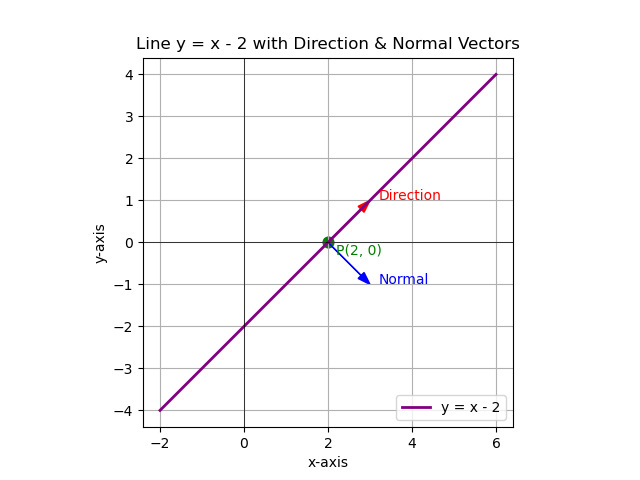
\includegraphics[width=0.6\columnwidth]{Figs/Fig1.png}
\end{center}
\caption{}
\label{fig:Fig.1}
\end{figure}

\end{document}
